\documentclass{article}
\usepackage{fullpage,subfigure,fancyhdr}
\usepackage[pdftex]{color}
\usepackage{wrapfig}
\usepackage{textcomp}
\usepackage{verbatim}
\usepackage{times}
\usepackage{amsfonts,amsmath,amssymb,amsthm}
\usepackage{textcomp}
\usepackage{url}
\usepackage{mdwlist}
\usepackage{subfigure}
\usepackage{sidecap}
\usepackage{wrapfig}
\usepackage{xspace}
\usepackage{algorithm,algorithmic}
\usepackage[pdftex]{graphicx}
\usepackage[colorlinks=true,pagebackref,linkcolor=magenta]{hyperref}
\usepackage[sort&compress,comma,round,numbers]{natbib}
\usepackage{pict2e}
\usepackage[nottoc,numbib]{tocbibind}
\usepackage{paralist}
\usepackage{multicol}
\usepackage{lettrine}
\usepackage{lineno}
% \usepackage{trackchanges}
% \usepackage{mcode}

\usepackage{helvet}
\renewcommand{\familydefault}{\sfdefault}
\definecolor{MyGray}{rgb}{0.7,0.7,0.7}

% \numberwithin{figure}{section}
% \numberwithin{table}{section}
% \numberwithin{algorithm}{section}


%%%%% COLOR STUFF %%%%%%%%%%
\newcommand{\db}[1]{{\color{dark_blue}{#1}}}
\newcommand{\bb}[1]{{\textbf{\db{#1}}}}

\definecolor{MyPlum}{rgb}{0.3,0,0.3}
\definecolor{MyOrange}{rgb}{1,0.5,0}
\definecolor{deep_blue}{rgb}{0,.2,.5}
\definecolor{dark_blue}{rgb}{0,.15,.5}

\newcommand{\marta}[1]{{\color{red}{\it marta: #1}}}
\newcommand{\youngser}[1]{{\color{green}{\it youngser: #1}}}
\newcommand{\brett}[1]{{\color{blue}{\it brett says: #1}}}
\newcommand{\jovo}[1]{{\color{magenta}{\it JoVo: #1}}}
\newcommand{\rb}[1]{{\color{red}{\it rb: #1}}}
\newcommand{\bro}[1]{{\color{blue}{\it youngser: #1}}}
\newcommand{\agastya}[1]{{\color{red}{\it agastya: #1}}}
\providecommand{\tg}[1]{\textcolor{green}{#1}}
\providecommand{\tb}[1]{\textcolor{blue}{#1}}
\providecommand{\tr}[1]{\textcolor{red}{#1}}
\providecommand{\tk}[1]{\textcolor{black}{#1}}
\providecommand{\twhite}[1]{\textcolor{white}{#1}}


%%%%%%%%% MATH OPERATORS %%%%%%%%%%%%
\providecommand{\ve}[1]{\boldsymbol{#1}}
\providecommand{\ma}[1]{\boldsymbol{#1}}
\providecommand{\norm}[1]{\left \lVert#1 \right  \rVert}
\providecommand{\deter}[1]{\lvert #1 \rvert}
\providecommand{\abs}[1]{\left \lvert #1 \right \rvert}
\providecommand{\mat}[1]{\left[ #1 \right]}
\newcommand{\trans}[1]{{#1}^{\ensuremath{\mathsf{T}}}}           % transpose
\newcommand{\transpose}[1]{{#1}^{\ensuremath{\mathsf{T}}}}           % transpose
\newcommand{\argmax}{\operatornamewithlimits{argmax}}
\newcommand{\argmin}{\operatornamewithlimits{argmin}}
\newcommand{\T}{^{\ensuremath{\mathsf{T}}}}           % transpose
\newcommand{\from}{{\ensuremath{\colon}}}           % :
\newcommand{\trace}[1]{{\ensuremath{\operatorname{tr}\!\left(#1\right)}}}           % :

\providecommand{\ms}[1]{\mathsf{#1}}
\providecommand{\mc}[1]{\mathcal{#1}}
\providecommand{\mb}[1]{\boldsymbol{#1}}
\providecommand{\mbb}[1]{\mathbb{#1}}
\providecommand{\mv}[1]{\vec{#1}}
\providecommand{\mh}[1]{\hat{#1}}
\providecommand{\wh}[1]{\widehat{#1}}
\providecommand{\mhv}[1]{\mh{\mv{#1}}}
\providecommand{\mvh}[1]{\mv{\mh{#1}}}
\providecommand{\mt}[1]{\widetilde{#1}}
\providecommand{\mhc}[1]{\hat{\mathcal{#1}}}
\providecommand{\mbc}[1]{\mb{\mathcal{#1}}}
\providecommand{\mvc}[1]{\mv{\mathcal{#1}}}
\providecommand{\mtc}[1]{\widetilde{\mathcal{#1}}}
\providecommand{\mth}[1]{\mt{\mh{#1}}}
\providecommand{\mht}[1]{\mh{\mt{#1}}}
\providecommand{\mhb}[1]{\hat{\boldsymbol{#1}}}
\providecommand{\whb}[1]{\widehat{\boldsymbol{#1}}}
\providecommand{\mvb}[1]{\vec{\boldsymbol{#1}}}
\providecommand{\mtb}[1]{\widetilde{\boldsymbol{#1}}}
\providecommand{\mbt}[1]{\widetilde{\boldsymbol{#1}}}
\providecommand{\mvc}[1]{\vec{\mathcal{#1}}}
% \newcommand{\D}[2]{\frac{\partial #1}{\partial #2}}
\newcommand{\dd}[2]{\frac{\partial ^2 #1}{\partial #2 ^2}}
\newcommand{\DDD}[3]{\frac{\partial ^2 #1}{\partial #2 \partial #3}}
\newcommand{\Di}[2]{\frac{\partial ^i #1}{\partial #2 ^i}}



%%%%%%%%%% SECTIONS & STUFF %%%%%%%%%%%%%

\newtheorem{Rem}{Remark}%[section]
\newtheorem{Alg}{Algorithm}%[section]
\newtheorem{thm}{Theorem}
\newtheorem{lem}{Lemma}
\newtheorem{Thm}{Theorem}[section]
\newtheorem{Lem}{Lemma}%[section]
\newtheorem{defi}{Definition}
\newtheorem{Def}{Definition}[section]
\newtheorem{prop}{Proposition}
\newtheorem{coro}[thm]{Corollary}
\newtheorem{claim}{Claim}
\newtheorem{conj}{Conjecture}
\newtheorem{question}{Question}
\newtheorem{rem}{Remark}%[section]
\newtheorem{cor}[lem]{Corollary}
\newtheorem{model}{Model}

\newcommand{\bla}{\begin{block}}
\newcommand{\blb}{\end{block}}

\newcommand{\defa}{\begin{defi}}
\newcommand{\defb}{\end{defi}}
\newcommand{\theHalgorithm}{\arabic{algorithm}}

\newcommand{\thma}{\begin{thm}}
\newcommand{\thmb}{\end{thm}}

\newcommand{\mata}{\begin{bmatrix}}
\newcommand{\matb}{\end{bmatrix}}

\floatname{algorithm}{Procedure}
\renewcommand{\algorithmicrequire}{\textbf{Input:}}
\renewcommand{\algorithmicensure}{\textbf{Output:}}
\floatname{algorithm}{Pseudocode}



%%%%%% section stuff %%%%%%%%%%
\renewcommand{\thesection}{\Roman{section}}   % set the section counter to Alpha
\renewcommand{\thesubsection}{\Roman{section}.\Alph{subsection}}   % set the subsection counter to alpha
% \renewcommand{\thesubsubsection}{\Alph{section}.\arabic{subsection}(\arabic{subsubsection})}   % set the subsection counter to alpha
% 
% 
\makeatletter
% \def\subsize{\@setsize\subsize{8pt}\xipt\@xipt}
 \def\section{\@startsection {section}{1}{\z@}{5pt}{9pt}{\Large\bf\db}}
 \def\subsection{\@startsection {subsection}{2}{\z@}{10pt}{4pt}{\large\bf\db}}
 \def\subsubsection{\@startsection {subsubsection}{2}{\z@}{10pt}{4pt}{\bf\db}}
% \def\subs{\@startsection {subsubsection}{2}{0pt}{5pt}{0pt}{ \subsize\bf\db}}
\def\paragraph{\@startsection {paragraph}{2}{\z@}{10pt}{4pt}{\bf\db}}
% \def\subparagraph{\@startsection 


\newcommand{\para}[1]{\vspace{3pt}\noindent{{\fontsize{11pt}{1em} \bf #1}}}
\newcommand{\subpara}[1]{\vspace{3pt}\noindent{{\fontsize{11pt}{1em} \bf \emph{#1}}}}
\newcommand{\subsubpara}[1]{\vspace{3pt}\noindent{{\fontsize{10pt}{1em} \emph{#1}}}}


%%%%%% SHORT HAND %%%%%%%%%%
\renewcommand{\refname}{References and Notes}

\newcommand{\jv}{Joshua Vogelstein}
\newcommand{\jhu}{Johns Hopkins University}
\newcommand{\website}{http://jovo.me/}
\newcommand{\email}{jovo@jhu.edu}

\newcommand{\Vr}{V_{reset}}
\newcommand{\Vl}{V_{leat}}
\newcommand{\eqdef}{\overset{\triangle}{=}}
\newcommand{\grad}{\nabla}
\newcommand{\Hess}{\nabla\nabla}
\newcommand{\defn}{\overset{\triangle}{=}}

\newcommand{\iid}{\overset{iid}{\sim}}
\newcommand{\knn}{$k$NN}

\newcommand{\elegans}{\emph{C. elegans} }

\newcommand{\Lik}{\mathcal{L}}
\newcommand{\Cae}{[\widehat{\text{Ca}}^{2+}]}
\newcommand{\Cav}{\ve{C}}%[\ve{\text{Ca}}^{2+}]}
\newcommand{\sml}{\sqrt{\ma{\lambda}}}
\newcommand{\ml}{\ma{\lambda}}
\newcommand{\nw}{\widehat{n}}
\newcommand{\nv}{\vec{n}}
\newcommand{\Ae}{\widehat{A}}
\newcommand{\te}{\widehat{\tau}}
\newcommand{\maxn}{\max_{\ve{n}: n_t \geq 0}}
% \newcommand{\V}{\text{Var}}

\newcommand{\PmcP}{P \in \mc{P}}
\newcommand{\mP}{\mathbb{P}}

% \newcommand{\dvs}{\dot{\bs}_t}
% \newcommand{\dvw}{\dot{\bw}_t}
% \newcommand{\dvx}{\dot{\bx}_t}
% \newcommand{\dvy}{\dot{\by}_t}

\newcommand{\ft}{f_{\ve{\thet}}}
\newcommand{\gt}{g_{\ve{\thet}}}
\newcommand{\hht}{h_{\thetn}}

\newcommand{\Real}{\mathbb{R}}



\newcommand{\wconv}{\overset{i.p.}{\rightarrow}}
\newcommand{\sconv}{\overset{i.p.}{\rightarrow}}
\newcommand{\conv}{\rightarrow}
\newcommand{\pconv}{\overset{p}{\conv}}
\newcommand{\mcE}{\mathcal{E}}
\newcommand{\mcT}{\mathcal{T}}
\newcommand{\mcG}{\mathcal{G}}
\newcommand{\mcM}{\mathcal{M}}
\newcommand{\mcL}{\mathcal{L}}
\newcommand{\hatmcE}{\widehat{\mcE}}
\newcommand{\hatp}{\widehat{p}}
\newcommand{\hatP}{\widehat{P}}
\newcommand{\hatQ}{\widehat{Q}}
\newcommand{\hatL}{\widehat{L}}
\newcommand{\mhP}{\widehat{\PP}}
\newcommand{\tildeA}{\widetilde{A}}
\newcommand{\defeq}{\overset{\triangle}{=}}


\DeclareMathOperator{\Pmat}{\mathbf{P}}
\DeclareMathOperator{\veta}{\mathbf{\mb{v}}}
\DeclareMathOperator*{\minimize}{\mathrm{minimize}}
\DeclareMathOperator*{\maximize}{\mathrm{maximize}}
% \DeclareMathOperator*{\mb{v}mod}{\mathbf{\mb{v}}}


%%%%%%% LATIN LETTERS


\newcommand{\bA}{\mb{A}}
\newcommand{\bB}{\mb{B}}
\newcommand{\bI}{\mb{I}}
\newcommand{\bP}{\mb{P}}
\newcommand{\bS}{\mb{S}}
\newcommand{\bU}{\mb{U}}
\newcommand{\bV}{\mb{V}}
\newcommand{\bW}{\mb{W}}
\newcommand{\bX}{\mb{X}}
\newcommand{\bY}{\mb{Y}}

\newcommand{\ba}{\mb{a}}
\renewcommand{\ba}{\mb{b}}
\newcommand{\bp}{\mb{p}}
\newcommand{\bs}{\mb{s}}
\newcommand{\bu}{\mb{u}}
\newcommand{\bv}{\mb{v}}
\newcommand{\bw}{\mb{w}}
\newcommand{\bx}{\mb{x}}
\newcommand{\by}{\mb{y}}


\newcommand{\Aa}{\mathbb{A}}
\newcommand{\BB}{\mathbb{B}}
\newcommand{\CC}{\mathbb{C}}         
\newcommand{\DD}{\mathbb{D}}         
\newcommand{\EE}{\mathbb{E}}           % expected value
\newcommand{\FF}{\mathbb{F}}         
\newcommand{\GG}{\mathbb{G}}
\newcommand{\HH}{\mathbb{H}}         
\newcommand{\II}{\mathbb{I}}           % indicator function
\newcommand{\LL}{\mathbb{L}}
\newcommand{\MM}{\mathbb{M}}
\newcommand{\NN}{\mathbb{N}}
\newcommand{\PP}{\mathbb{P}}         
\newcommand{\QQ}{\mathbb{Q}}           
\newcommand{\SSS}{\mathbb{S}}           
\newcommand{\VV}{\mathbb{V}}
\newcommand{\WW}{\mathbb{W}}         
\newcommand{\XX}{\mathbb{X}}         
\newcommand{\YY}{\mathbb{Y}}
\newcommand{\ZZ}{\mathbb{Z}}         




\newcommand{\Qs}{Q}
\newcommand{\mcS}{\mc{S}}
\newcommand{\mcU}{\mc{U}}

\newcommand{\mbd}{\mb{d}}
\newcommand{\mbD}{\mb{D}}
\newcommand{\mbx}{\mb{x}}
\newcommand{\mbX}{\mb{X}}
\newcommand{\mby}{\mb{y}}
\newcommand{\mbY}{\mb{Y}}

\newcommand{\mtbd}{\mtb{d}}
\newcommand{\mtbD}{\mtb{D}}
\newcommand{\mtbx}{\mtb{x}}
\newcommand{\mtbX}{\mtb{X}}
\newcommand{\mtby}{\mtb{y}}
\newcommand{\mtbY}{\mtb{Y}}



\DeclareMathOperator{\Ri}{\mathbf{\R}^{-1}}
\DeclareMathOperator{\A}{A}
\DeclareMathOperator{\W}{\mathbf{W}}
\DeclareMathOperator{\V}{\mathbf{V}}
\DeclareMathOperator{\U}{\mathbf{U}}
\DeclareMathOperator{\C}{\mathbf{C}}
\DeclareMathOperator{\uvec}{\mathbf{u}}
\DeclareMathOperator{\D}{\mathbf{D}}
\DeclareMathOperator{\Q}{\mathbf{Q}}
\DeclareMathOperator{\R}{R} %\mathbf{P}}
\DeclareMathOperator{\Y}{\mathbf{Y}}
\DeclareMathOperator{\B}{\mathbf{B}}
\DeclareMathOperator{\Hmat}{\mathbf{H}}
\DeclareMathOperator{\Gmat}{\mathbf{G}}
\DeclareMathOperator{\X}{\mathbf{X}}
\DeclareMathOperator{\Cmat}{C} %\mathbf{L}}\providecommand{\ms}[1]{\mathsf{#1}}

\DeclareMathOperator*{\Ymod}{\mathbf{\Y}}
\DeclareMathOperator*{\Bmod}{\mathbf{B}}
\DeclareMathOperator*{\Hmod}{\mathbf{H}}
\DeclareMathOperator*{\Lmod}{\mathbf{L}}
\DeclareMathOperator*{\Xmod}{\mathbf{\X}}


%%% THETA %%%%

\newcommand{\bth}{\ve{\theta}}
\newcommand{\hth}{\mh{\theta}}
\newcommand{\htth}{\mh{\theta}}
\newcommand{\bhth}{\mh{\ve{\theta}}}
\newcommand{\thetn}{\ve{\theta}}
\newcommand{\thet}{\thetn}
\newcommand{\theth}{\widehat{\ve{\theta}}}
\newcommand{\theto}{\ve{\theta}'}
\newcommand{\wht}{\widehat{\thet}}
\newcommand{\wtt}{\widetilde{\thet}}
\newcommand{\vth}{\ve{\thet}}
\newcommand{\vTh}{\ve{\Theta}}
\newcommand{\hvth}{\widehat{\ve{\thet}}}
\newcommand{\bTh}{\ve{\Theta}}
\newcommand{\hbth}{\widehat{\thet}}
\newcommand{\tbth}{\tilde{\bth}}



% \newcommand{\p}{P_{\bth}}
\newcommand{\pold}{P_{\bth'}}
\newcommand{\pk}{P_{\widehat{\ve{\theta}}^{(k)}}}
\newcommand{\pT}{P_{\thetn_{Tr}}} %\thetn_T
\newcommand{\pO}{P_{\thetn_o}} %\thetn_o
% \newcommand{\Q}{Q(\thetn,\theto)}
% \newcommand{\m}{m^{\ast}}
% \newcommand{\q}{q(\ve{H}_t)}
\newcommand{\Ca}{[\text{Ca}^{2+}]}


%%%%%% GREEK LETTERS

\newcommand{\del}{\delta}
\newcommand{\sig}{\sigma}
\newcommand{\lam}{\lambda}
\newcommand{\gam}{\gamma}
\newcommand{\eps}{\varepsilon}

\newcommand{\Del}{\Delta}
\newcommand{\Sig}{\Sigma}
\newcommand{\Lam}{\Lambda}
\newcommand{\Gam}{\Gamma}

\newcommand{\bSig}{\ve{\Sigma}}
\newcommand{\bOm}{\ve{\Omega}}
\newcommand{\bLam}{\ve{\Lambda}}
\newcommand{\bPhi}{\ve{\Phi}}
\newcommand{\bPsi}{\ve{\Psi}}

\newcommand{\bmu}{\ve{\mu}}
\newcommand{\bal}{\ve{\alpha}}
\newcommand{\bpi}{\ve{\pi}}
\newcommand{\bkap}{\ve{\kappa}}
\newcommand{\bdel}{\ve{\delta}}
\newcommand{\bphi}{\ve{\phi}}
\newcommand{\bpsi}{\ve{\psi}}



\DeclareMathOperator{\Delti}{\mathbf{\Delta}^{-1}}
\DeclareMathOperator{\Delt}{Q} %\mathbf{\Delta}}
% \DeclareMathOperator{\Gam}{\mathbf{\Gamma}}
\DeclareMathOperator{\Gami}{\mathbf{\Gamma}^{-1}}
\DeclareMathOperator{\Sigb}{\mathbf{\Sigma}}






%%%%%%%%%%% ALGORITHM NAMES %%%%%%%%%%%%%

\newcommand{\FAQ}{\texttt{FAQ} }

\providecommand{\sct}[1]{{\sc \texttt{#1}}}
\newcommand{\msl}{{\sc Idt}}

\newcommand{\Svd}{\sct{Svd}}
\newcommand{\Pca}{\sct{Pca}}
\newcommand{\Fld}{\sct{Fld}}
\newcommand{\Lda}{\sct{Lda}}
\newcommand{\eig}{\sct{eig}}
\newcommand{\qr}{\sct{qr}}
\newcommand{\Lol}{\sct{Lol}}
\newcommand{\Lal}{\sct{Lal}}
\newcommand{\Lrl}{\sct{Lrl}}
\newcommand{\Lfl}{\sct{Lfl}}





\title{\vspace{-50pt}
% Reliable and Reproducible Brain-Based Measures for Candidate Biomarker Discovery from Big Data
% Optimal Discovery Science from Big Brain-Imaging Data via Reliability and Reproducibility  
\db{Optimal Detection and Design via Maximizing Discriminability: \\ Applications in Neuroimaging}
}
\author{Shangsi Wang, Zhi Yang, Xi-Nian Zuo, Michael Milham, Cameron Craddock,  \\ 
Greg Kiar, William Gray Roncal, Eric Bridgeford,
Consortium for Reliability and Reproducibility, \\ Carey E.~Priebe, Joshua T. Vogelstein}


\begin{document}

\maketitle
\tableofcontents
\newpage

\section{Introduction}

\para{Opportunity and Challenge} In this era of big data, many scientific, government, and corporate groups are collecting and processing massive datasets. To obtain optimal quantitative answers to any inquiry about data requires making two decisions: (i) “how should the data be collected?”, and (ii) “how should the data be processed?”  When the downstream inference task is specified, a priori, we can collect and process data to optimize the performance of task. However, recently, across industry, governmental, and academic settings, certain datasets become benchmark or reference datasets. Such datasets can then be used for a wide variety of different inferential problems.  Collecting and processing these datasets requires massive institutional investments, and choices related to questions(i) and (ii) above have dramatic effects on all subsequent analyses. Optimally addressing experimental design decisions can yield significant savings in both the financial and human costs, and also improve accuracy of analytical results. Therefore, a theoretical framework to enable investigators to select from a set of possible design decisions using pilot data could reap great rewards



\para{Action and Resolution} 
To this end, we have proposed and developed a formal definition of discriminability to guide data collection and processing. Discriminability is a non-parametric statistical property of a joint distribution in a hierarchical model, to differentiate between classes of objects. We prove that discriminability (which may be more aptly called reliability), provides a lower bound on predictive accuracy for any downstream inference task, even if we have never seen the covariates to predict. We then design an estimator of discriminability computed from test-restest data set, demonstrate that it is unbiased, and derive our estimator’s asymptotic distribution. 

Numerical simulations are conducted to demonstrate the basic property of our discriminability estimator in a variety of settings. Then, we apply our approach to choose amongst a set of choices one must make when designing a neuroimaging study to specifically study functional connectomics. We start by finding the maximally reliable threshold for converting correlation matrices  into graphs. Indeed, consistent with our theoretical and simulated results,
maximizing the discriminability of our datasets also maximizes performance on a suite of different downstream inference tasks. We then ask about a series of pre-processing steps: should one motion correct or not, and
should one implement global signal regression or not, etc. We determine the optimal choice for each pre-processing steps, and find the maximally discriminable pipelines amongst 64 pre-processing pipelines.

Thus, in total, our discriminability analysis is a powerful tool for making decisions about how to collect and analyze
datasets designed for discovery science. We expect this method to be useful in a wide variety of applications,
and therefore have made all the code open source and available from http://openconnecto.
me.




\section{Results}



\subsection{Theory}

\subsubsection{Definition of Discriminability}
 Discriminability measures the overall consistency and differentiability of observations. For example, if a subject is measured twice under the same conditions, two observations should be close to each other given the measure is consistent. In addition, one should be able to tell these two observations come from the same subject when compared to observations from other subjects given the measure is differentiable. We quantify this idea of consistency and differentiability through discriminability. 
 
To formalize the definition of discriminability, consider the following generative process. For each sample $i$, there exists some true physical property $\bv_i$. Unfortunately, we do not get to directly observed $\bv_i$, rather, we measure it with some device, that transforms the truth from $\bv_i$ to $\bw_i$ via $f_{\bphi}$.  The parameter $\bphi \in \bPhi$ characterizes all options in the measurement, including, for example, which scanner to use, which resolution, the number of images, sampling rate, etc.  The output of $f_{\bphi}$ is the  ``raw'' observation data $\bw_i$, but it is corrupt in various ways, including movement or intensity artifacts introduced by the measurement process.  Therefore, rather than operating directly on $\bw_i$, we intentionally ``pre-process'' the data, in an effort to remove a number of nuisance variables.  This pre-processing procedure further transforms the data from $\bw_i$ to $\bx_i$ via $g_{\bpsi}$.   The parameter $\bpsi \in \bPsi$ indexes all pre-processing options, including whether to perform motion correction, which motion correction, deconvolution, etc.  More specifically, the entire code base, including dependencies, and even the hardware the pre-processing is running on, could count as $\bpsi$. For brevity, we define $\bx_i:= g_{\bpsi} \big(f_{\bphi} (\bv_i) \big)$.

Let $i$ denote the sample's unique \emph{identity} (hereafter, referred to as the \emph{subject}) and $t$ denote the trial number.  Thus, there is a single $\bv_i$ for subject $i$, but we have $\bw_{i,t}$, which is the $t^{th}$ trial, implicitly also a function of $\bphi$, which encodes all the details of the measurement. If both $f$ and $g$ together do not introduce too much noise, then we would expect that $\bx_{i,1}$ and $\bx_{i,2}$ are \emph{closer} to one another than either are to any other subject's data, $\bx_{i',t}$.  Define $\delta$ to be a metric computing the distance between two data points, $\delta \from \mc{X} \times \mc{X} \to \Real_+$.  Formally, we expect that $\delta(\bx_{i,t},\bx_{i,t'}) \leq \delta(\bx_{i,t},\bx_{i',t''})$, for any $i,i',t,t',t''$.  
For brevity, let $\delta_{i,t,t'}:=\delta(\bx_{i,t}, \bx_{i,t'})$ and 
$\delta_{i,i',t,t''}:=\delta(\bx_{i,t}, \bx_{i',t''})$.  
This intuition leads to our definition of discriminability:
\begin{align}
D(\bpsi,\bphi) = \PP[ \delta_{i,t,t'} \leq \delta_{i,i',t,t''}]
\end{align}
When trying to find the best pre-processing routine encoded by $\bpsi$, we try to maximize the discriminability of processed data, that is 
\begin{equation} 
\begin{aligned}
& \underset{\bpsi \in \bPsi}{\text{maximize}}
& & D(\bpsi,\bphi)
\end{aligned}
\end{equation}


\subsubsection{Optimizing discriminability Optimizes Bound on Performance for Any Task}

Consider the situation that the downstream task is classification, that is in addition to $\bv_i$, there are other properties of sample $i$ of interest; we call all of them $\by_i \in \mc{Y}$.  These may include, for example, the phenotype of the subject, including personality tests, demographic information, and genetic data. The goal of experimental design, in this context, is to choose $\bphi \in \bPhi$ and $\bpsi \in \bPsi$ to make prediction of $\by_i$ based on $\bx_i$ easier. 

To quantify the performance of our choice, we introduce some assumptions.  First, assume that each $(\bv_i,\by_i)$ pair is sampled independently and identically from some distribution, $(\bv_i,\by_i) \iid F_{V,Y}$.  For simplicity, let us assume that our goal is binary classification, using $\bx_i$ as the \emph{predictor} variables, and a binary-valued $\by_i$ as the \emph{target} variable. Moreover, the loss function, $\ell$ quantifies the Bayes classification error
\[\ell( \bx_i, \by_i) =  \PP(C^{B}(\bx_i) \neq \by_i)\]
 Here, $C^{B}(\bx_i)= \underset{y_i \in \{0,1\} }{\text{argmax }} \PP(\by_i=y|\bx_i) $ . Under some assumptions, we can prove theorem 1 which asserts that Bayes classification error is bounded by an decreasing function of discriminability. 
\begin{thm}	
	There is a decreasing function $h$, such that
\[\ell( \bx_i, \by_i) \leq h(D(\bpsi,\bphi)) \]
\end{thm}

Therefore, we expect the classification performance to be better when the more discriminable processing pipeline is used. This theorem justifies
maximizing discriminability of processed data improves prediction accuracy.

\subsubsection{Estimator/Test Statistic}
In practice, exact distribution of $\bx_{i,t}$ may never known to us; hence, it is not possible to compute discriminability $D(\bpsi,\bphi)$ or $D$ in short when there is no ambiguity in processing pipelines under consideration. However, samples $x_{i,t}$ are observed, and we can approximate true discriminability using an estimator $\hat{D}$ which is a function of observed samples. For each pair of observations $x_{i,t}$ and $x_{i,t'}$ from the same subject $i$, we first define
\[ \hat{D}_{i,t,t'} = \frac{\sum\limits_{i' \neq i}^{n} \sum\limits_{t''=1}^{s} \mathbb{I}\{\delta_{i,t,t'} \leq \delta_{i,i',t,t''} \} }{(n-1)s}\]
Here, $n$ is the total number of subjects, and $s$ is the number of observations per subject. $\hat{D}_{i,t,t'}$ approximate the probability that distance between observations from other subjects and $t^{th}$ observation of subject $i$ is larger than distance between $t^{th}$ and $t'^{th}$ trial of subject $i$. Then, we define $\hat{D}$ to be the mean of $\hat{D}_{i,t,t'}$.
\[ \hat{D} := \frac{\sum\limits_{i=1}^{n} \sum\limits_{t=1}^{s}  \sum\limits_{t' \neq t}^{s} \hat{D}_{i,t,t'}}{ns(s-1)} \]
$\hat{D}$ serves as the sample approximated discriminability. The next lemma asserts the unbiasedness of $\hat{D}$ as an estimator.

\begin{lem}	
	\[ E(\hat{D}) = D\]
\end{lem}

The following lemma shows the as the number of subjects increase, $\hat{D}$ converges in probability to discriminability.
\begin{lem}	
As $n \rightarrow \infty$,
\[\hat{D} \overset{p}{\rightarrow} D \]
\end{lem}

\subsection{Simulations}

\subsubsection{Convergence of $\hat{D}$}
In Lemma 1 and 2, we assert sample discriminability $\hat{D}$ is unbiased and converges to  the true population discriminability in probability. We demonstrate this idea with simulation. The true physical property are generated from independent Gaussian distribution. That is $v_i \overset{i.i.d.}{\sim} \mathbb{G}(0,1)$. All subjects have two observations with additive noise: $x_{i,t} | v_i \sim \mathbb{G}(v_i,1)$. For each number of subjects, we generate data and compute discriminability 100 times. 

The figure 1 shows how $\hat{D}$ is distributed when we vary the sample size from 10 to 200. With this data generation scheme, the population discriminability can be computed from numerical integration, and is marked on the plot. We can see from the figure that sample discriminabiity $\hat{D}$ converges to $D$ as sample size increase.

\begin{figure}[t!]
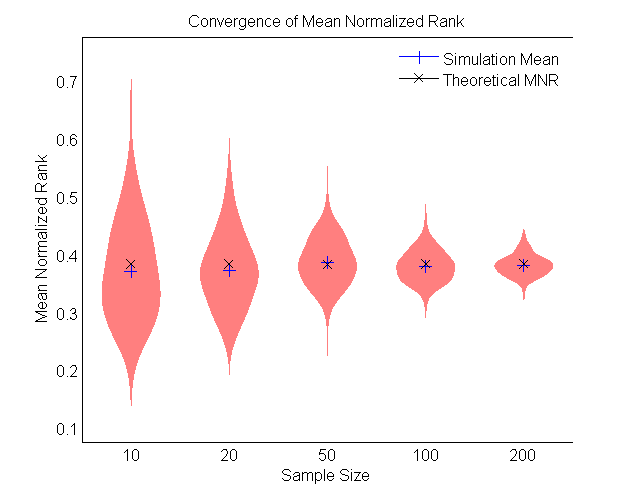
\includegraphics[width=3.0in]{../Figs/simumnr_violin.png}
\caption{{\bf Convergence of sample Discriminability.} As the number of samples increases, the sample Discriminability  converges to true population Discriminability }
\label{fig:1}
\end{figure}




\subsubsection{Dhat provides a more useful bound than ICC or I2C2 for a variety of simulated settings}

\begin{figure}[t!]
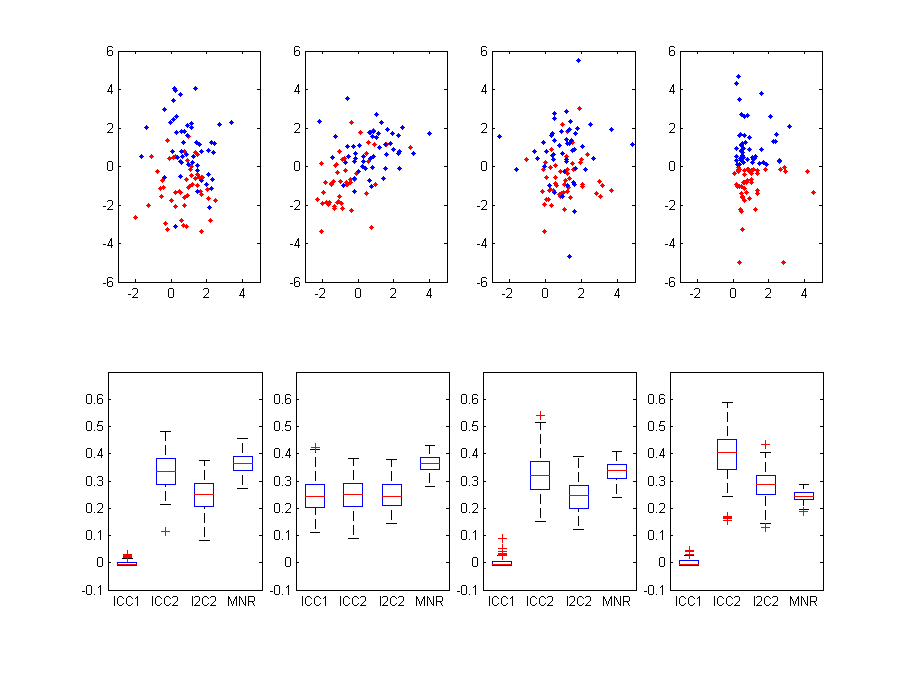
\includegraphics[width=3.0in]{../Figs/Figure1_draft.png}
\caption{Two class ICC, I2C2 and Discriminability}
\label{fig:2}
\end{figure}



\subsubsection{we can use Dhat to choose the most discriminable parameter (eg, threshold)}


\begin{figure}[t!]
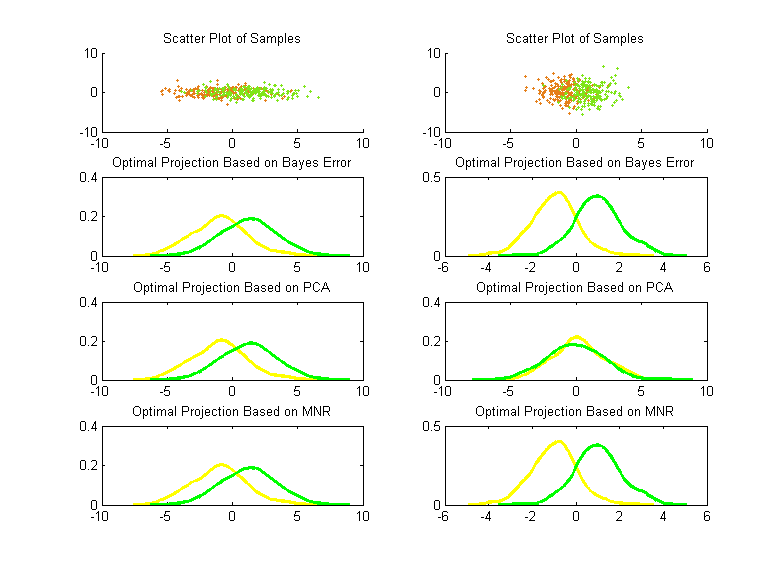
\includegraphics[width=3.0in]{../Figs/parameter_selection_2sub.png}
\caption{{\bf Best linear projection selected by PCA and Discriminability.} Best linear projections are computed based on PCA and optimizing Discriminability. Under two settings, maximizing Discriminability always yields Bayes optimal projection. }
\label{fig:3}
\end{figure}




\subsection{Connectome Applications}

\subsubsection{optimal Discriminability yields optimal predictive accuracy}
\begin{itemize}
\item Introduce how fmri graph is constructed
\item Describe how we threshold correlation and what is being predicted, how we predict
\item explain the result in fig 4 that maximal discriminability yields best prediction performance 
\end{itemize}

\begin{figure}[t!]
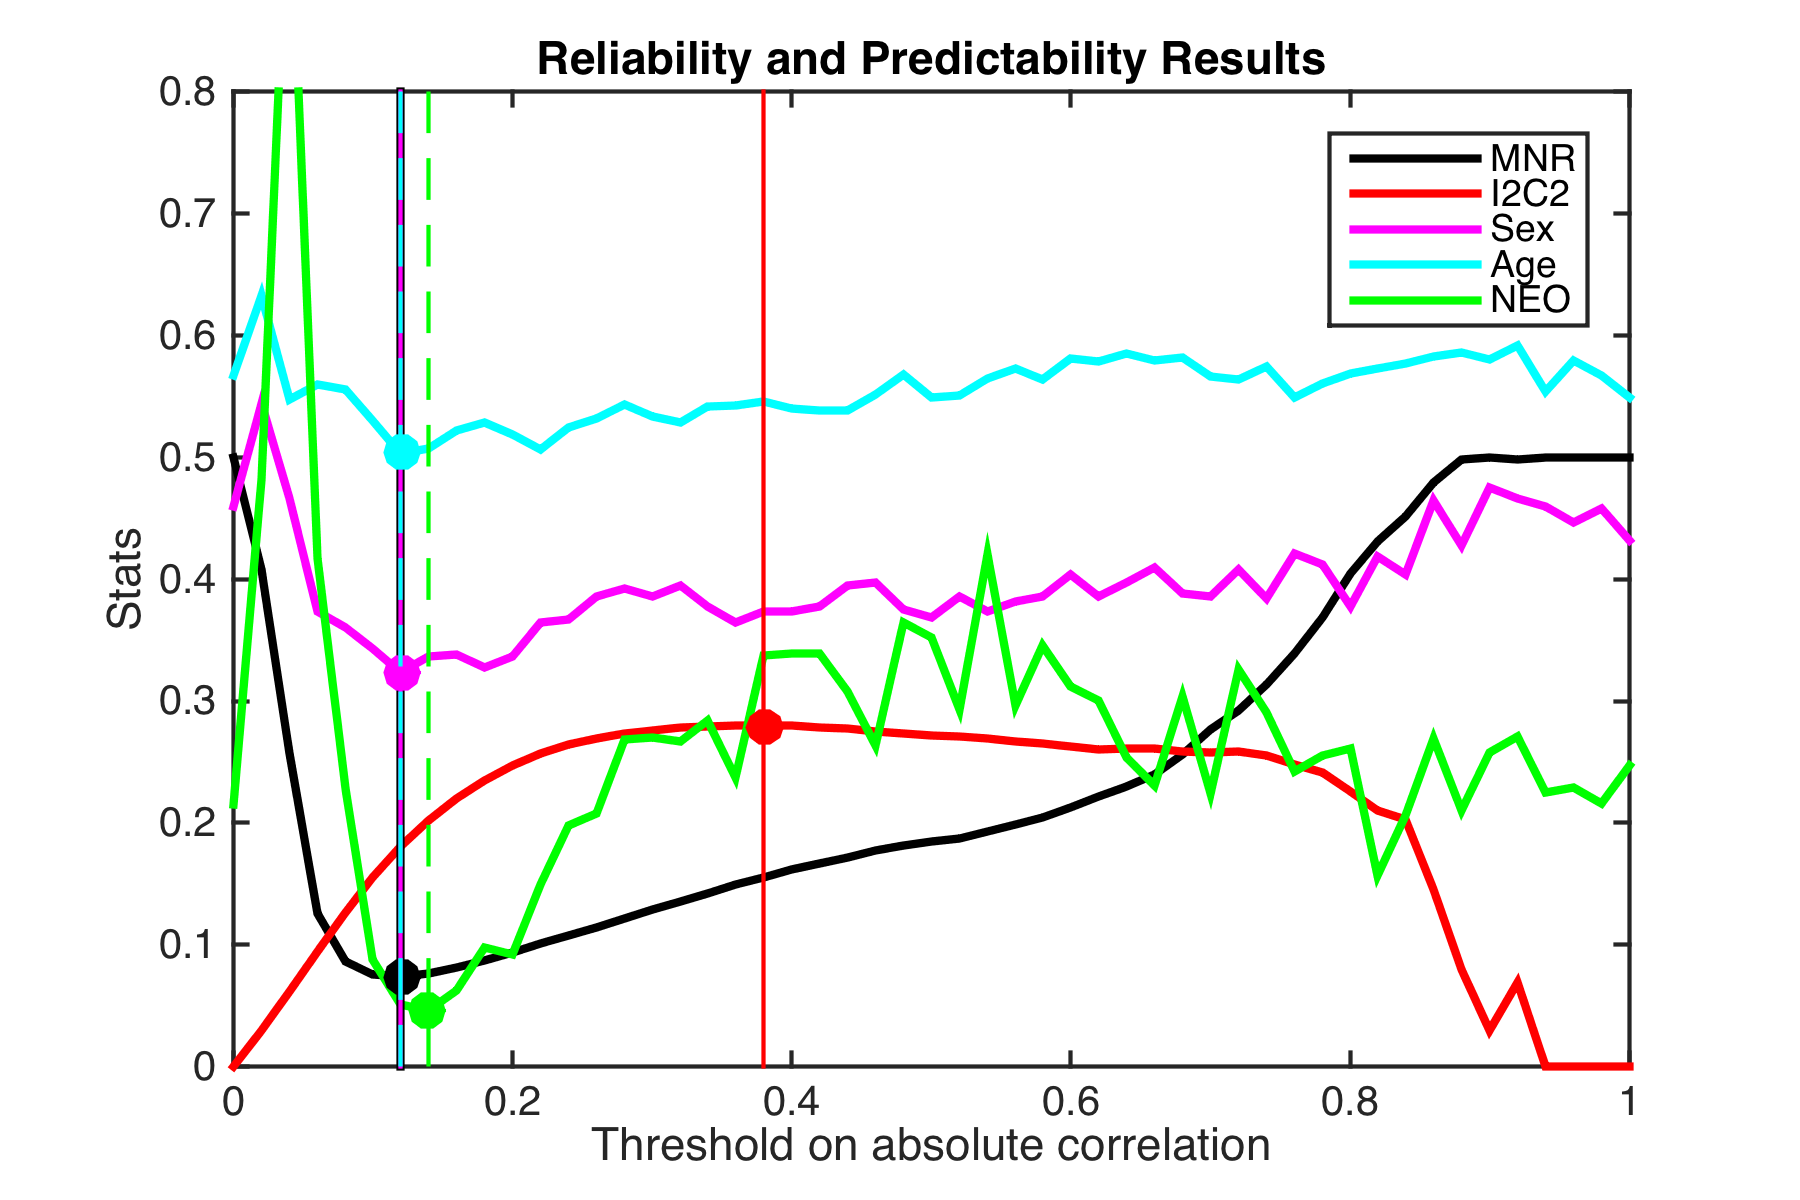
\includegraphics[width=3.0in]{../Figs/HCP.png}
\caption{{\bf Optimizing Discriminability yields optimal prediction accuracy for gender and age.} The raw correlation graph is thresholded to convert it to a binary graph. The threshold is varied from 0 to 1. At each threshold, the discriminability is computed; gender and age are predicted using k-NN. The threshold maximizing discriminability yields optimal prediction performance for both covariates. }
\label{fig:4}
\end{figure}

\begin{figure}[t!]
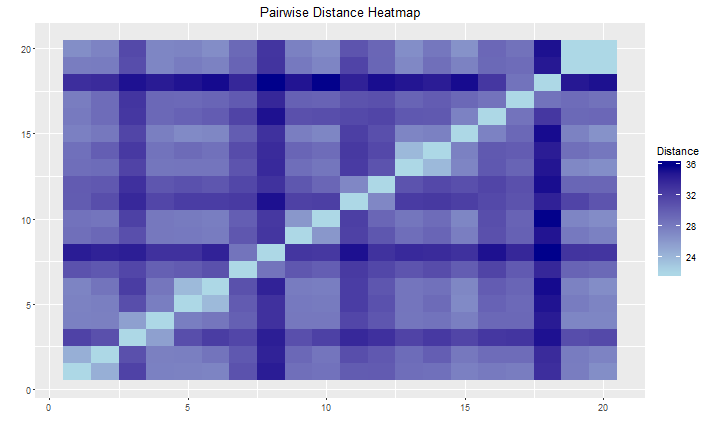
\includegraphics[width=3.0in]{../Figs/pairdistance.png}
\caption{{\bf Pairwise distance of an discriminable data set.} Pairwise distance of 20 observations from 10 subjects are displayed. The observations are from BNU1 data set processed by CFXXG pipeline. The small 2-by-2 block on the diagonal indicates that within subject distance is smaller than across subject distance. }
\label{fig:5}
\end{figure}


\subsubsection{Best Pipeline of 64 (raw correlation graph)}
\begin{itemize}
	\item Explain the problem of finding the best pipelines
	\item Explain what four decisions are  and 4 atlases, nff vs frf, fsl vs ant, scrub vs no scr, gsr vs no gsr. 
	\item Claim we find the best pipeline with maximum mean (without a hypothesis tesing)
\end{itemize}

\begin{figure}[t!]
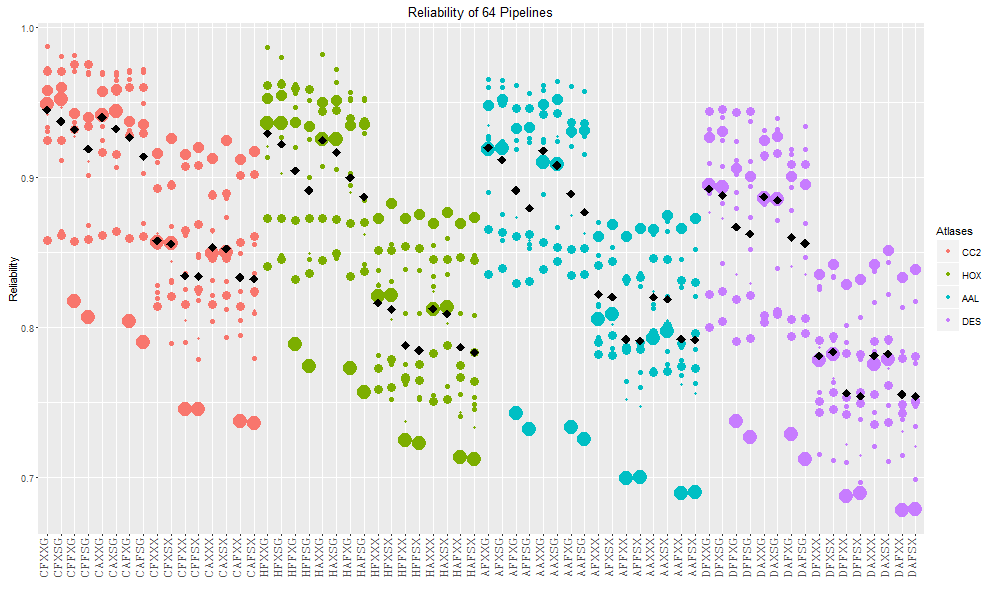
\includegraphics[width=3.0in]{../Figs/64_pipelines_size.png}
\caption{{\bf Discriminability of raw fmri graphs from 12 data sets processed 64 ways.}  Discriminability of BNU1, BNU2, DC1, IACAS, IBATRT, IPCAS, JHNU, NYU1, SWU1, UM, UWM and XHCUMS processed by 64 pipelines are computed. CFXXG pipeline has the best mean Discriminability across data set. }
\label{fig:6}
\end{figure}


\subsubsection{best pipeline = product of marginals}
\begin{itemize}
	\item Explain we focus on individual decision for statistical significance
	\item Explain how we perform the multifactor analysis of variance test
	\item we find nff better than frf, fsl better than ant, scrub ? no scr, gsr better than no gsr, and atlas is being significant, best pipeline = product of marginals
\end{itemize}

\begin{figure}[t!]
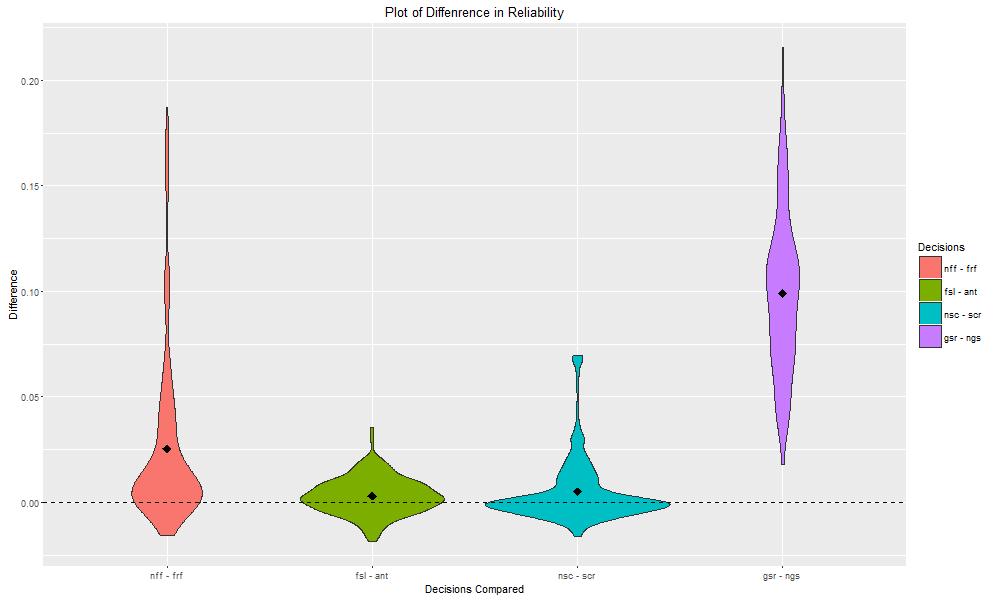
\includegraphics[width=3.0in]{../Figs/Differ_violin_mean.png}
\caption{{ \bf Paired difference in Discriminability of each decisions.} Difference in Discriminability for each decision is compared by fixing other decisions and a data set. nff, fsl and gsr is statistical significantly better. }
\label{fig:7}
\end{figure}

\subsubsection{which atlas/resolution}
\begin{itemize}
	\item Background info about 4 atlases
	\item claim cc200 better than hox  better than aal better than des
\end{itemize}

\subsubsection{rank graphs}

\begin{itemize}
	\item Explain how rank graphs are constructed, the motivation to robust estimate graphs
	\item Explain it offers large improvement over raw fmri graphs when there is no gsr, small when there is gsr.s
\end{itemize}
\begin{figure}[t!]
	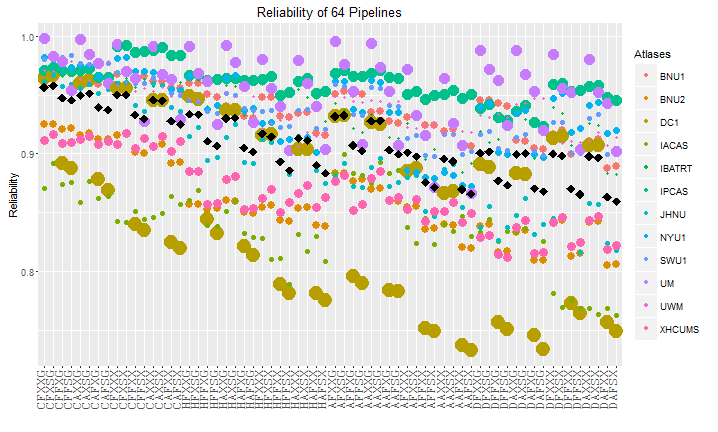
\includegraphics[width=3.0in]{../Figs/64_pipelines_size_rank.png}
	\caption{{\bf Discriminability of rank fmri graphs from 12 data sets processed 64.} Discriminability of same data sets are computed with correlation graphs converting into rank graphs. CFXSG is the best pipeline in terms of mean Discriminability.}
	\label{fig:8}
\end{figure}


\begin{figure}[t!]
	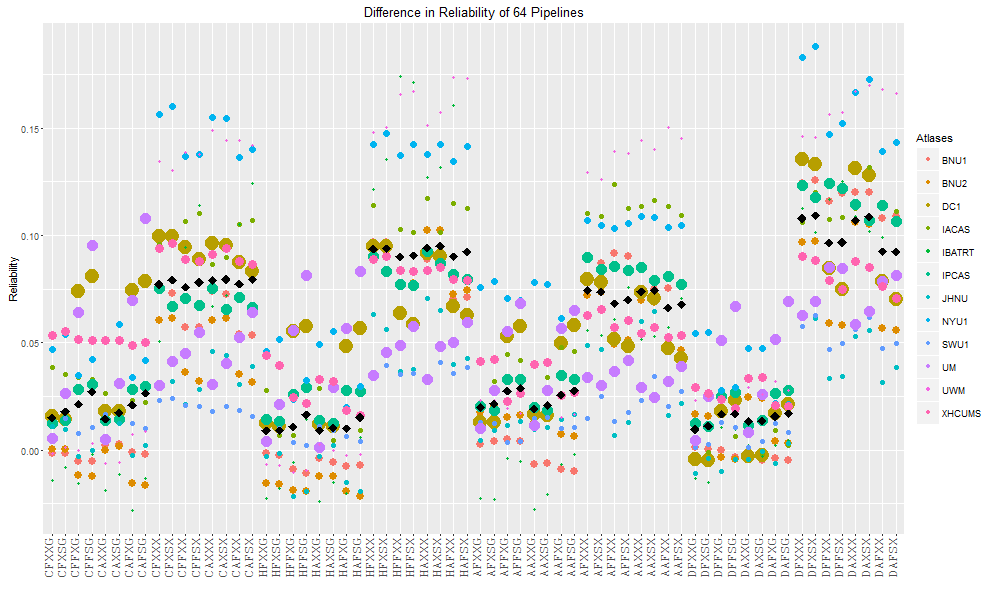
\includegraphics[width=3.0in]{../Figs/64_pipelines_differ.png}
	\caption{{\bf Difference in Discriminability of rank vs raw fmri graphs from 12 data sets processed 64.} Difference in discriminability is computed by fixing a pipeline and a data set. Overall, rank graphs is more discriminable than raw correlation graphs, especially when no global signal regression is performed. }
	\label{fig:9}
\end{figure}




\subsubsection{DTI vs. fMRI}










\section{Discussion}

\para{Summary}

\para{Related Work}
Our discriminability statistics is not the first attempt to quantify information of test-retest data set. Previous works include but not limit to: analysis of variance (ANOVA), intraclass correlation coefficient (ICC), image intraclass correlation coefficient (I2C2) and distance components (DISCO). The ANOVA and ICC approaches only operate on scalar data set. I2C2 is a generalization of ICC into high dimension space, however it is designed for additive Gaussian noise and assumes Euclidean distance. DISCO is a statistics designed to test whether multi-modal distribution are the same or not. It is less robust and intuitive compared to $\hat{D}$. Also, the mean of DISCO varies with the number of subject and dimension of observation which makes it not suitable to compare across data set.


\para{Next Steps}


% \input{intro}
% \input{simulations}
% \input{flow}
% \input{setting}
% \input{logic}
% \input{main}
% \input{setup}
% \input{gRAICAR}



\appendix






\newpage
\small{
\bibliography{biblio}
\bibliographystyle{IEEEtran}
}


\end{document}
